\documentclass{amsart}
\usepackage{graphicx}
\graphicspath{{./}}
\usepackage{hyperref}
\usepackage{csvsimple}
\usepackage{longtable}
\usepackage{lscape}
\usepackage{epigraph}
\title{Ethnicity Effects on Stealing Is Justified}
\author{Zulfikar Moinuddin Ahmed}
\date{\today}
\begin{document}
\maketitle

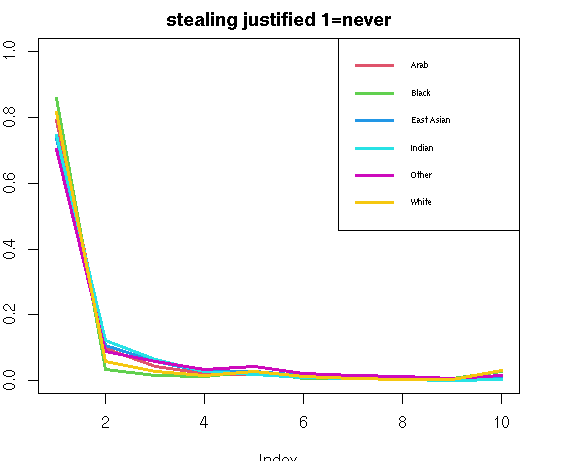
\includegraphics[scale=0.8]{steal.png}

\section{Mass Concentrated in 1-6}

% latex table generated in R 4.0.3 by xtable 1.8-4 package
% Fri May 14 22:03:33 2021
\begin{table}[ht]
\centering
\begin{tabular}{rr}
  \hline
 & mass6 \\ 
  \hline
Arab & 0.98 \\ 
  Black & 0.95 \\ 
  East Asian & 0.97 \\ 
  Indian & 0.99 \\ 
  Other & 0.95 \\ 
  White & 0.95 \\ 
   \hline
\end{tabular}
\end{table}

\section{Exponential Fits}

% latex table generated in R 4.0.3 by xtable 1.8-4 package
% Fri May 14 22:09:36 2021
\begin{table}[ht]
\centering
\begin{tabular}{rlrr}
  \hline
 & eth & lambda & rsq \\ 
  \hline
1 & Arab & 0.58 & 0.87 \\ 
  2 & Black & 0.32 & 0.40 \\ 
  3 & East Asian & 0.51 & 0.87 \\ 
  4 & Indian & 0.64 & 0.91 \\ 
  5 & Other & 0.38 & 0.76 \\ 
  6 & White & 0.36 & 0.52 \\ 
   \hline
\end{tabular}
\end{table}

Here $\sigma(\lambda)=0.13
$ is the variation due to ethnicity in the exponential decay with mean 
\[
\mu(\lambda)=0.47
\]
The variation is quite negligibly small, as we can see from the total mass concentration of people in 1-6.

\section{Strengths of Inference From Sample Sizes}

Our inferences are based on samples $N \ge 1100$ for all ethnicity classes.  These are more than enough to overcome various small sample biases.

% latex table generated in R 4.0.3 by xtable 1.8-4 package
% Fri May 14 22:48:03 2021
\begin{table}[ht]
\centering
\begin{tabular}{rr}
  \hline
 & N \\ 
  \hline
Arab & 1144 \\ 
  Black & 2084 \\ 
  East Asian & 8964 \\ 
  Indian & 2560 \\ 
  Other & 27783 \\ 
  White & 6820 \\ 
   \hline
\end{tabular}
\end{table}

\section{Grand Conclusion}

The burden lies on those who have ethnic theories of morality to explain the uniformity in human race convictions about stealing, say, across the globe.  Our conclusions about irrelevance of morality in human race comes from extremely strong regularities in the distributions of all ethnicities. The effect of ethnicity is rather small on the force here of Human Nature, and I would not want to take on any position on ethnic differences on morality after examining the data.  The data are strong and overwhelming, and ethnic theories of morality would be attempting to find something significant in noise.  Theories of ethnic differences in morality were political propaganda from Europe in the seventeenth to nineteenth century that never had any scientific merit, and we can dismiss them as not just pseudo-scientific but totally wrong and misguided today with high quality data.  Ethnic theories of morality belong with all other junk fantasies of primitive ages as a fascinating irrational phenomenon and historical curiosity now.

This conclusion is not just from this note but a larger ouvre of my work on these topics.  I am able to offer the Markov Moral Model which explains around 91\% of the variability of morality of the Human Race, leaving around 9\% to ethnicity and other effects.  

Now 9\% is scientifically not trivial, but we live on the threshold of an age which had theorised incessantly not just in Europe but in Asia about all manner of creative fantasies about superior morality of one tribe or another.  So I am not enthusiastic about entering this labyrinth of error and confusion at the moment.  Arthur de Gobineau was so enthusiastic about this erroneous path that he wrote a thick tome claiming 'race' will explain everything.  We have better truth; human race, who I am rather fond of, is a noble race indeed, and has a bright future without all these primitive superstitions about tribal supremacy and other drivel.


\end{document}